% Add your research tags below (comma-separated, case-insensitive)
% Year is automatically added as a tag
% 2025: 2025
%<TOPICs>:  graphical models 


\documentclass[11pt,letterpaper]{article}

\newcommand{\workingDate}{\textsc{2025 $|$ September $|$ 20}}
\newcommand{\userName}{Research Student}
\newcommand{\institution}{University} 

\usepackage{assets/styles/diary_base}        % Core packages and basic theorems
\usepackage{assets/styles/diary_theorems}   % Enhanced colored theorem environments (optional)
\usepackage{assets/styles/diary_commands}   % Personal shortcuts and commands


\begin{document}
\href{run:2025-09-20.tex}{\Huge September 20} %##@@TitleDateString@@##

\section*{Reflow}

\begin{figure}[h]
\centering 
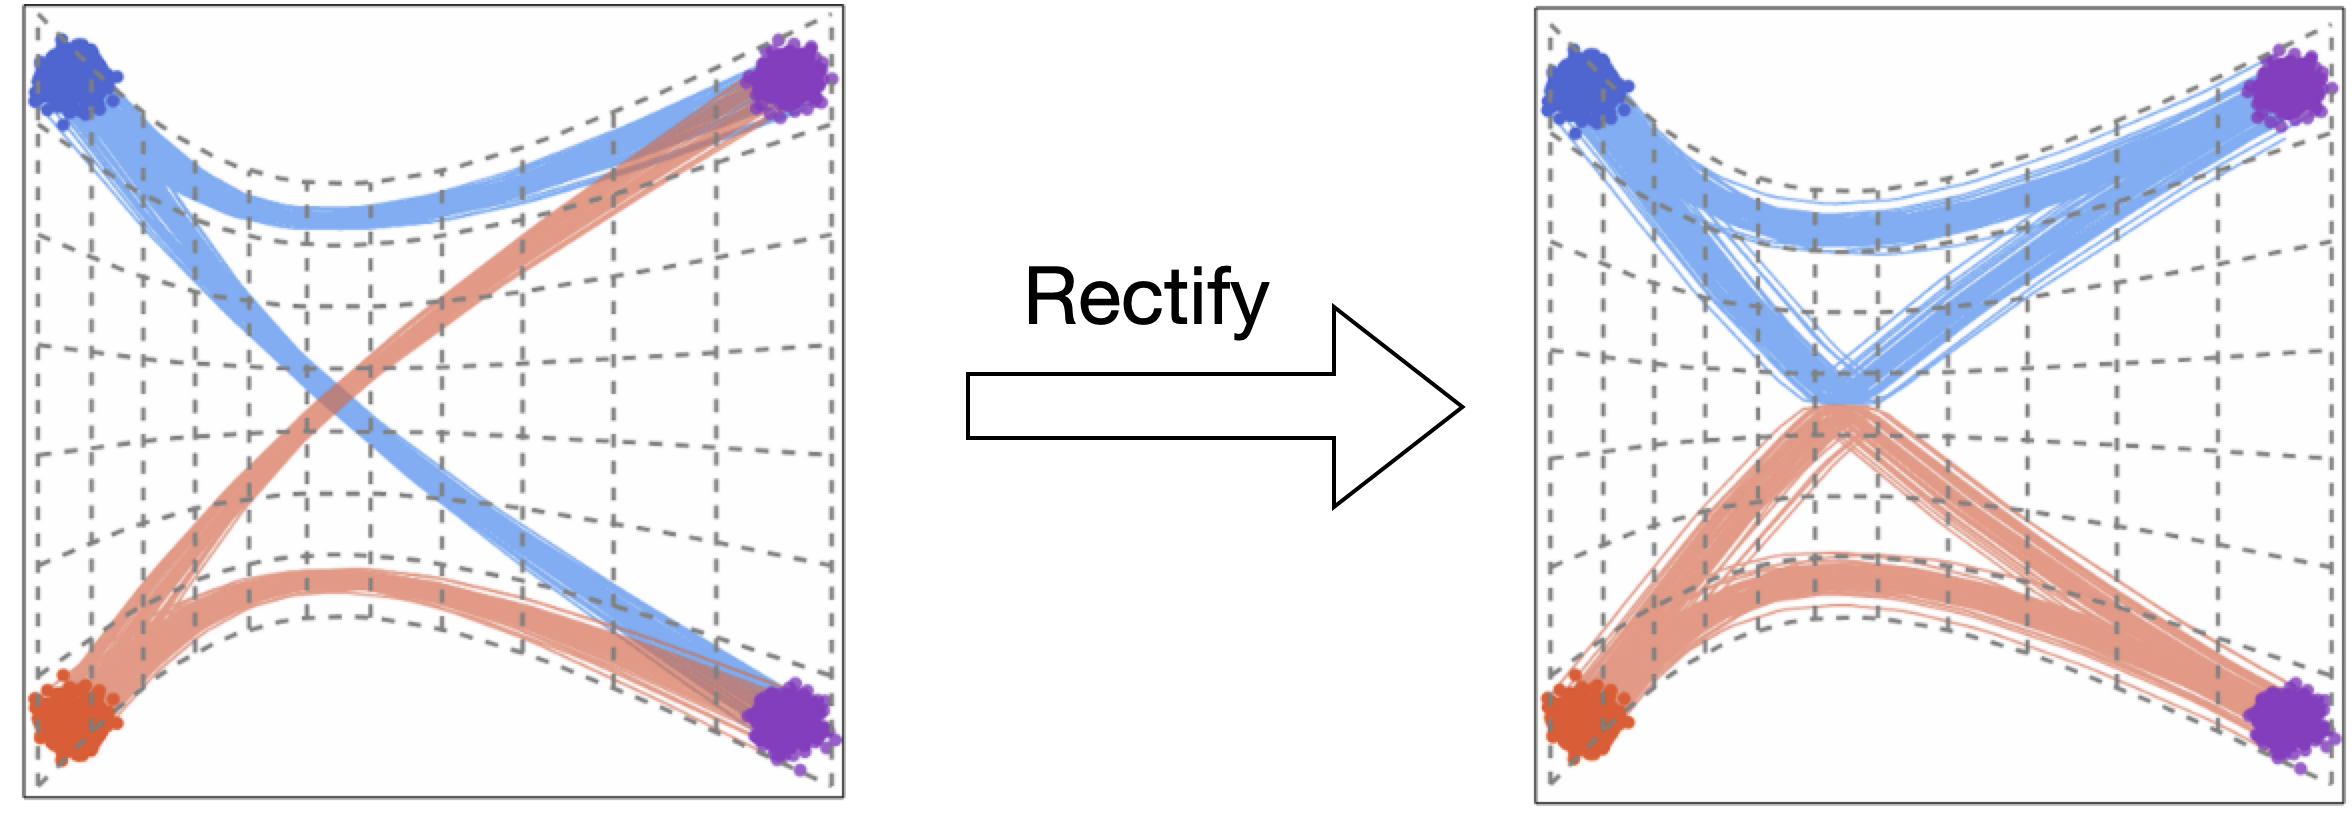
\includegraphics[width=0.8\textwidth]{assets/figures/2025/curved_reflow.png}
\end{figure} 


Yes. I want to cite \cite{li2022diffusion}. 


\bibliographystyle{apalike} 
\bibliography{assets/bibliography/z}%##@@BibFileString@@##
\end{document}
